\documentclass[letterpaper,twocolumn,openany,nodeprecatedcode]{dndbook}

\usepackage[italian]{babel}
%\usepackage[italian]{babel}
% For further options (multilanguage documents, hypenations, language environments...)
% please refer to babel/polyglossia's documentation.

\usepackage[utf8]{inputenc}
\usepackage[singlelinecheck=false]{caption}
\usepackage{lipsum}
\usepackage{listings}
\usepackage{shortvrb}
\usepackage{ragged2e}
\usepackage{stfloats}
\usepackage{graphicx} % Add this package for image support
\usepackage{tcolorbox} % Aggiungi questo pacchetto

\captionsetup[table]{labelformat=empty,font={sf,sc,bf,},skip=0pt}

\MakeShortVerb{|}

\lstset{%
  basicstyle=\ttfamily,
  language=[LaTeX]{TeX},
  breaklines=true,
}

\title{\sc Andata e Ritorno:\\ il viaggio di Semestra per le terre di Thylea}
\author{\sc Giacomo}
\date{\today}

\begin{document}

\frontmatter

\maketitle

\tableofcontents

\mainmatter%

\chapter*{Prologo}
\justifying
\DndDropCapLine{S}{emestra vide la luce} in una fredda alba d’inverno, il 30 Gennaio 1463 C.V., 
alle pendici delle Montagne della Spada, nella Foresta del Giardino delle Cripte, un luogo intriso 
di mistero e leggende. La foresta, con i suoi alberi secolari e le radure avvolte da una nebbia 
perenne, sembrava quasi voler custodire il segreto della sua nascita. Kristen, sua madre, era una 
giovane hobbit dal sangue nobile, figlia di uno dei capi dei Pugni Fiammanti, la temuta milizia di 
Baldur's Gate. Ma il suo destino era stato segnato da un’onta che non poteva essere cancellata. 
Vittima di un atto di violenza da parte del suo stesso padre, Kristen si trovò a portare in grembo 
una vita che non aveva scelto, ma che non poteva sopprimere. La vergogna e il disonore che 
gravavano sulla sua famiglia la spinsero a compiere una scelta dolorosa: abbandonare la neonata 
alle pendici delle Montagne della Spada, lontano dagli occhi giudicanti della società.

\DndDropCapLine{N}{on fu il destino}, né la volontà degli dèi, a guidare Thorin verso quel fragile fagotto avvolto in 
una coperta logora. Thorin, un nano delle Montagne e fedele della Vecchia Fede, venerava la Natura 
come unica entità soprannaturale, rifiutando ogni altra divinità. Era un druido, un tempo un fiero 
guerriero che aveva combattuto contro Halaster il Mago Folle nelle profondità di Undermountain. 
Dopo quella battaglia, segnato nel corpo e nello spirito, aveva deciso di abbandonare la vita di 
avventuriero per dedicarsi alla cura della Foresta Alta, devastata dalle maledizioni scagliate da 
Halaster. Nel suo piccolo insediamento naturalistico, nascosto tra le colline e protetto dalla 
magia della natura, Thorin trovò in Semestra una nuova ragione di vita. La prese con sé, nutrendola 
con latte di capra e raccontandole, fin dai suoi primi giorni, le storie degli antichi eroi e delle 
terre selvagge. La foresta divenne la sua culla, i canti degli uccelli il suo ninna nanna, e le mani 
callose di Thorin il suo rifugio sicuro. 

\section{Un incontro inaspettato}

\DndDropCapLine{L}{’addestramento di Semestra} sotto la guida di Thorin non fu privo di difficoltà. 
Fin dai primi anni, la giovane mostrò una certa avversione verso la magia. Nonostante gli sforzi 
del druido, Semestra non riusciva a padroneggiare neanche i più semplici incantesimi. 
Ogni tentativo di evocare la magia sembrava scivolarle via, come sabbia tra le dita. 
Frustrata, ma determinata a non deludere il suo mentore, Semestra si dedicò con passione alle 
altre arti druidiche. Imparò il druidico, la leggendaria lingua segreta dei druidi, 
usata per comunicare con la natura e per tracciare rune magiche. 
Tuttavia, anche queste rune sembravano prive di potere quando tracciate dalle sue mani, 
un fatto che alimentava in lei un senso di inadeguatezza.\\

Fu solo all’età di sedici anni, durante la sua prima pattuglia solitaria nella Foresta Alta, 
che il destino decise di rivelare il suo potenziale. Mentre camminava tra gli alberi secolari, 
immersa nei suoni della natura, Semestra si imbatté in un piccolo topo ferito. Il minuscolo 
animale giaceva immobile tra le foglie, il suo pelo bianco macchiato di sangue. 
La vista di quel fragile essere in difficoltà colpì profondamente il cuore della giovane. 
Si inginocchiò accanto al topo, le lacrime che le rigavano il viso. Lo prese delicatamente 
tra le mani, sentendo il suo respiro debole e irregolare. Una lacrima, cadendo dal suo viso, 
scivolò sul pelo del topo.\\

\begin{figure}[h!]
  \begin{tcolorbox}[
      enhanced,
      colframe=PhbTan,      % Usa il colore lavanda predefinito del tema DMG
      colback=white,
      opacityback=0,
      title={\vspace{0.2cm}\centering \sc  \textbf{Semestra e Larry}\vspace{0.2cm}},
      colbacktitle=PhbTan!50!PhbLightCyan,
      coltitle=black,
      fonttitle=\bfseries
  ]
  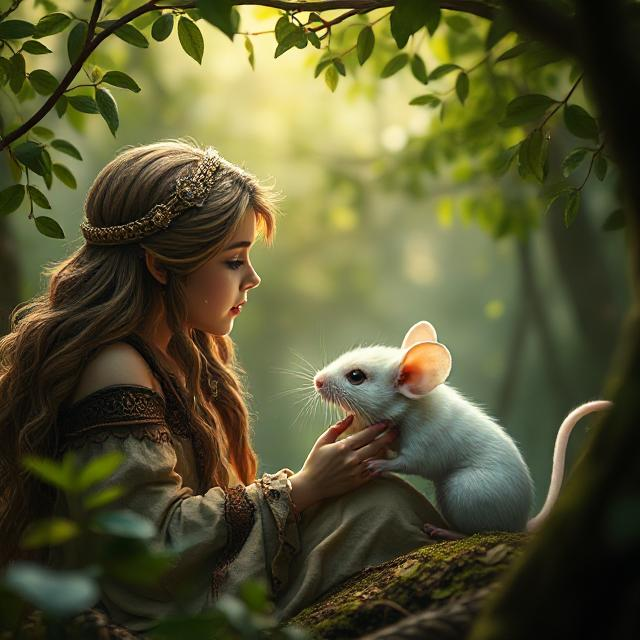
\includegraphics[width=\textwidth]{img/semestra_larry-1.jpeg}
  \label{fig:semestra-larry}
  \end{tcolorbox}
\end{figure}

\DndDropCapLine{F}{u allora} che accadde qualcosa di straordinario. La lacrima, non appena toccò 
il piccolo animale, brillò di una luce calda e dorata. Semestra osservò incredula mentre il topo 
si rianimava, le sue ferite si chiudevano e il suo respiro tornava regolare. Era il suo primo 
incantesimo: \textit{Cura Ferite}. In quel momento, Semestra comprese che la magia non era qualcosa che poteva essere forzata o appresa con la sola disciplina. Era un dono, un legame profondo con la natura, che si manifestava solo quando il cuore e l’anima erano in perfetta armonia. Il topo, ora guarito, si arrampicò sulla sua spalla, come per ringraziarla, e da quel giorno divenne il suo fedele compagno, un simbolo del suo legame con la natura e del potere che finalmente aveva scoperto dentro di sé.

\begin{figure*}[b]
    \begin{tcolorbox}[
        enhanced,
        colframe=PhbTan,
        colback=white,
        opacityback=0,
        title={\vspace{0.2cm}\centering \sc  \textbf{La mappa del Fear\"un}\vspace{0.2cm}},
        colbacktitle=PhbTan!50!PhbLightCyan,
        coltitle=black,
        fonttitle=\bfseries
    ]
    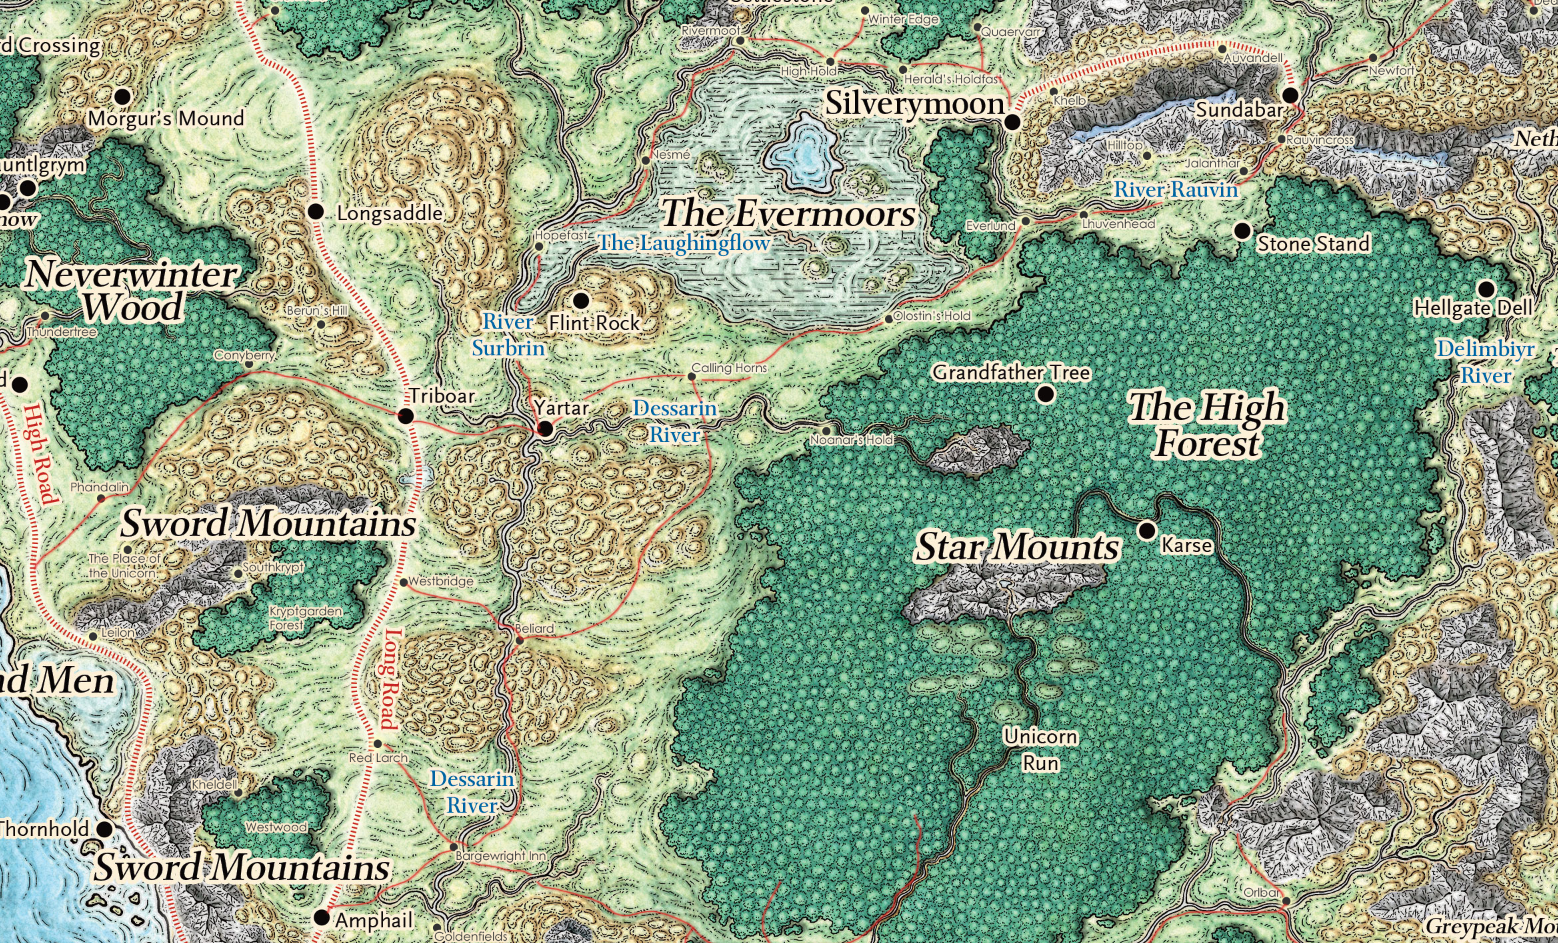
\includegraphics[width=\textwidth]{img/fearun_map.png}
    \caption{\centering La mappa del Fear\"un.}
    \label{fig:fearun-map}
    \end{tcolorbox}
\end{figure*}

Semestra sapeva che era proibito interferire con il corso naturale delle cose, così nascose il piccolo topolino, che poi chiamò Larry, finché non fu completamente guarito. Nonostante le regole della Vecchia Fede, sentiva che salvare quella fragile creatura era la cosa giusta da fare. Larry divenne presto il suo fedele compagno, un simbolo del suo legame con la natura e della sua crescente comprensione del mondo che la circondava.
\begin{DndMonster}[float*=b,width=\textwidth + 8pt]{Larry}
  \begin{multicols}{2}
    \DndMonsterType{Bestia, Taglia Minuscola, Neutrale Buono}

    % If you want to use commas in the key values, enclose the values in braces.
    \DndMonsterBasics[
        armor-class = {10 (armatura naturale)},
        hit-points  = {1 (\DndDice{1d4 - 1})},
        speed       = {6m},
      ]

    \DndMonsterAbilityScores[
        str = 2,
        dex = 11,
        con = 9,
        int = 10,
        wis = 10,
        cha = 4,
      ]

    \DndMonsterDetails[
        %saving-throws = {Str +0, Dex +0, Con +0, Int +0, Wis +0, Cha +0},
        %skills = {Acrobatics +0, Animal Handling +0, Arcana +0, Athletics +0, Deception +0, History +0, Insight +0, Intimidation +0, Investigation +0, Medicine +0, Nature +0, Perception +0, Performance +0, Persuasion +0, Religion +0, Sleight of Hand +0, Stealth +0, Survival +0},
        %damage-vulnerabilities = {cold},
        %damage-resistances = {bludgeoning, piercing, and slashing from nonmagical attacks},
        %damage-immunities = {poison},
        %condition-immunities = {poisoned},
        senses = {Scurovisione 9m, Percezione Passiva 10},
        languages = {Comprende il Comune},
        challenge = 0,
      ]
    % Traits
    \DndMonsterSection{Tratti}
    \DndMonsterAction{Olfatto Affinato} Larry ha vantaggio alle prove di Saggezza (Percezione) basate sull'olfatto.
    \DndMonsterSection{Actions}
    \DndMonsterAction{Multiattack}
    The foo makes two melee attacks.

    %Default values are shown commented out
    \DndMonsterAttack[
      name=Dagger,
      %distance=both, % valid options are in the set {both,melee,ranged},
      %type=weapon, %valid options are in the set {weapon,spell}
      mod=+3,
      %reach=5,
      %range=20/60,
      %targets=one target,
      dmg=\DndDice{1d4+1},
      dmg-type=piercing,
      %plus-dmg=,
      %plus-dmg-type=,
      %or-dmg=,
      %or-dmg-when=,
      %extra=,
    ]

    %\DndMonsterMelee calls \DndMonsterAttack with the melee option
    \DndMonsterMelee[
      name=Flame Tongue Longsword,
      mod=+3,
      %reach=5,
      %targets=one target,
      dmg=\DndDice{1d8+1},
      dmg-type=slashing,
      plus-dmg=\DndDice{2d6},
      plus-dmg-type=fire,
      or-dmg=\DndDice{1d10+1},
      or-dmg-when=if used with two hands,
      %extra=,
    ]

    %\DndMonsterRanged calls \DndMonsterAttack with the ranged option
    \DndMonsterRanged[
      name=Assassin's Light Crossbow,
      mod=+1,
      range=80/320,
      dmg=\DndDice{1d8},
      dmg-type=piercing,
      %plus-dmg=,
      %plus-dmg-type=,
      %or-dmg=,
      %or-dmg-when=,
      extra={, and the target must make a DC 15 Constitution saving throw, taking 24 (7d6) poison damage on a failed save, or half as much damage on a successful one}
    ]

    % Legendary Actions
    \DndMonsterSection{Legendary Actions}
    The foo can take 3 legendary actions, choosing from the options below. Only one legendary action option can be used at a time and only at the end of another creature's turn. The foo regains spent legendary actions at the start of its turn.

    \begin{DndMonsterLegendaryActions}
      \DndMonsterLegendaryAction{Move}{The foo moves up to its speed.}
      \DndMonsterLegendaryAction{Dagger Attack}{The foo makes a dagger attack.}
      \DndMonsterLegendaryAction{Create Contract (Costs 3 Actions)}{The foo presents a contract in a language it knows and waves it in the face of a creature within 10 feet. The creature must make a DC 10 Intelligence saving throw. On a failure, the creature is incapacitated until the start of the foo's next turn. A creature who cannot read the language in which the contract is written has advantage on this saving throw.}
    \end{DndMonsterLegendaryActions}
  \end{multicols}
\end{DndMonster}
\end{document}
